\documentclass[a4paper,10pt]{article}
\topmargin-1cm
\addtolength{\textheight}{2.5cm}
\addtolength{\textwidth}{2cm}
\usepackage{times}

\usepackage{verbatim}
\usepackage{color}
\usepackage{listings}
\usepackage{amsmath}
\usepackage{graphicx}
\usepackage[german]{babel}
\usepackage[latin1]{inputenc}

\setlength{\parindent}{0cm}

\title{Aufgabe 5 Programmieren HF-ICT}
\author{David Herzig}
\date{September 2017}

% some listings configurations:

\lstset{numbers=left,
        numberstyle=\tiny,
        keywordstyle=\color{blue}\bfseries\sffamily,
        identifierstyle=\ttfamily,
        commentstyle=\em,
        stringstyle=\ttfamily,
        extendedchars=true,
        showstringspaces=false,
        language=c++}
%

\renewcommand{\arraystretch}{2.0}

\begin{document}

HF-ICT - H"ohere Fachschule f"ur Informations- und Kommunikationstechnologie\\
Programmieren 3. Semester, Algorithmen und Datenstrukturen\\
David Herzig

\vspace{2mm}

\begin{center}
{\Large \bf Algorithmen und Datenstrukturen}\\
Exercise sheet 5
\end{center}

\vspace{2mm}

\line(1,0){400}

\vspace{5mm}

\section{Binary Search Tree}
Welcher bin"are Suchbaum entsteht bei den folgenden Operationen?
Wie sieht die Post-Order Traversierung aus?

\vspace{3mm}

insert(25), insert(47), insert(17), insert(10)\\
insert(19), insert(29), insert(26), insert(30)\\
remove(26), insert(82), remove(25), remove(17)

\vspace{3mm}

{\bf ACHTUNG:} Beim Remove soll immer das Element der linken Seite ber"ucksichtigt werden.


\section{Validierung}
Gegeben ist ein bin"arer Baum in Form eines Array. Das Element an Position 0 ist der Root Knoten.
Danach lassen sich die Child Nodes (Positionen im Array) eines Knoten wie folgt berechnen:

\begin{gather}
Node = i\\
Node.Left = 2 \cdot i + 1\\
Node.Right = 2 \cdot i + 2
\end{gather}

Der Array \verb|{20, 12, 34, 9, 19, 29}| ergibt den folgenden Baum:\\
\vspace{3mm}
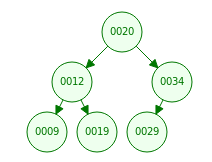
\includegraphics[scale=0.7]{tree}
\vspace{3mm}

Implementieren Sie eine Methode, welche einen Baum in Array Form bekommt. Diese Methode
liefert \verb|true|, falls es sich um einen bin"aren Suchbaum handelt. Falls es lediglich
ein bin"arer Baum ist, liefert die Methode \verb|false|.

\begin{lstlisting}
class TreeUtil {
public:
  static bool isBinarySearchTree(vector<int> values);
};
\end{lstlisting}

\section{Maximum Value}
Gegeben ist ein bin"arer Baum (nicht ein bin"arer Suchbaum) in Array Form. Finden Sie den Pfad
zum Blatt, bei welchem alle die Werte aller Nodes zusammengez"ahlt, maximiert wird.

\begin{lstlisting}
class TreeUtil {
public:
  static void printMaximumPath(vector<int> values);
};
\end{lstlisting}

Beispiel: Der Baum \verb|40, 100, 200, 20, 40, 70, 80, 50, 10| sieht wie folgt aus:\\
\vspace{3mm}
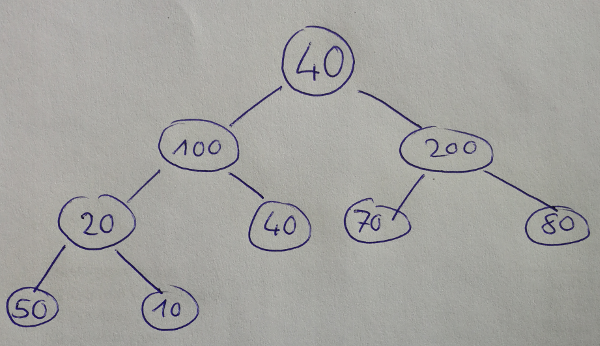
\includegraphics[scale=0.3]{tree2}
\vspace{3mm}

Die Ausgabe m"usste dann lauten: 40, 200, 80 (dieser Pfad ergibt die maximale Summe 320).	

\section{Sch"one Zeichenketten}
Die Sch"ohnheit einer Zeichenkette wird wie folgt definiert: Die Sch"onheit einer
Zeichenkette ist die Summe aller einzelnen Buchstaben, wobei jedem Buchstaben jeweils einen Wert
(1..26) zugeordnet wird. Nun gilt es, den Wert eines Buchstaben so zu bestimmen, dass die Summe aller Buchstaben
maximal ist. Es spielt dabei keine Rolle ob die Buchstaben gross oder klein geschrieben
sind.

\vspace{3mm}

Beispiele:\\
ABBCCC\\
Sometimes test cases are hard to make up.\\

\vspace{3mm}

Die erste Zeichenkette hat die Sch"onheit 152, die zweite Zeichenkette hat die
Sch"onheit 729.

\vspace{3mm}

Implementieren Sie eine Methode, welche die maximale Sch"obheit einer Zeichenkette
berechnet.

\vspace{3mm}

\begin{lstlisting}
int calculate(string input) {
  // your code
}
\end{lstlisting}

\end{document}

